\documentclass{beamer}

\usetheme[progressbar=frametitle]{metropolis}
\setbeamertemplate{frame numbering}[fraction]
\useoutertheme{metropolis}
\useinnertheme{metropolis}
\usefonttheme{metropolis}
\usecolortheme{spruce}
\setbeamercolor{background canvas}{bg=white}

\definecolor{mygreen}{rgb}{.125,.5.25}
\usecolortheme[named=mygreen]{structure}

\title[Basics OF UNIX]{TOPICS IN SOFTWARE SYSTEMS}
\subtitle{Chapter 1: Introduction to system programming}
\author{Sembatya Erios Naiga}
\date{2018/9/20}

\begin{document}

\begin{frame}
\titlepage
\end{frame}

\begin{frame}[t]{CONTENTS}\vspace{4pt}
\begin{enumerate}
\item Introduction
\item Unix architecture
\item Logging in
\item Files and directories
\item Input and output
\item Programs and processes
\item Error handling
\item User Identification
\item Signals
\item Time values
\item System Calls and Library Functions
\end{enumerate}

\end{frame}


\begin{frame}[t]{INTRODUCTION}\vspace{10pt}
\begin{enumerate}
\item Familiarize with UNIX
\item Fundamentals and Operating system concepts 
      \begin{enumerate}
      \item Multi-user concepts
      \item Basic and advanced I/O
      \item Process 
      \end{enumerate}       
\item Interprocess communication
\end{enumerate}

\end{frame}

\begin{frame}[t]{UNIX ARCHITECTURE}\vspace{10pt}
\begin{center}
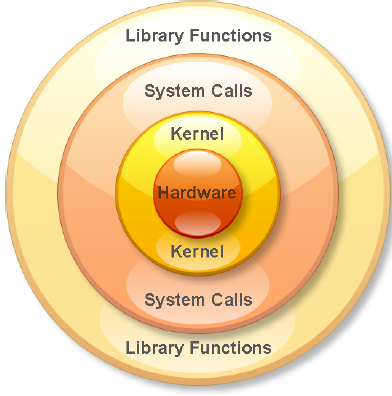
\includegraphics[scale=0.5]{kernel.png}
\end{center}
Figure 1: Architecture of UNIX operating system

\end{frame}


\begin{frame}[t]{UNIX ARCHITECTURE}\vspace{4pt}
\textbf{Kernel} is a software (SW) that controls the hardware (HW) of the computer and provides an environment under which programs can run (Figure 1).

\textbf{System calls:} are entry points inti which kernel codes where the functions are implemented.\\[6pt]
\textbf{Library calls (functios):} are transfers to user code with which performs the desired functions.

An \textbf{operating system (OS)} consists of the kernel and all other SWs that make a computer useful and gives the computer its personality. Other SW include system utilities, applications, shells, libraries of common functions etc. for example, for linux, kernel used by GNU OS is GNU(sometimes referred to as GNU linux OS) has an advantage of being more siccunt.

\end{frame}


\begin{frame}[t]{LOGGING IN}\vspace{10pt}
After log in, the system looks up for your login in its password file (/etc/passwd) which is composed of 7 colon separated fields (login name, encrypted password, user ID 205), numeric group ID (105), a comment field, home directory (/home/sar) and shell program (/bin/ksh). That is, sar: x: 205: 105: Sembaty Erios: home/sar: /bin/ksh. (chapter 6).

\textbf{Shell:} is a command-line interpreter that reads user input and executes commands. It is a special application that provides an interface for running other applications.

After log in, you type commands to the shell and the system knows which shell to execute for us based on the field in our entry password file. 

\end{frame}

\begin{frame}[t]{LOGGING IN}\vspace{10pt}
The system knows which shell to execute for us based on the final field in our entry in the password file.\\[10pt]\textbf{There are 5 common shells used} (chapter 2).

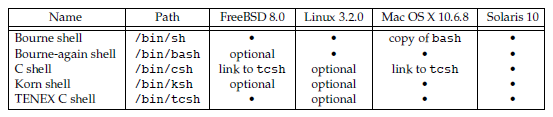
\includegraphics[scale=0.5]{shellstable.png}\\[6pt]
Figure 2: Common shells used on UNIX systems.


\end{frame}

\begin{frame}[t]{FILES AND DIRECTORIES}
\textbf{NOTE:} The research Unix system and some older Unix system v-file systems filenames are restricted to 14 characters. BSD versions – extended limit of 255 characters and almost all commercial Unix file systems support 255 character filenames.
\\[10pt]\textbf{Pathname:} A sequence of 1 or more filenames separated by slashes (relative pathname) and starting with a slash (an absolute pathname). Relative pathname files are relative to the current directory.

\end{frame}


\begin{frame}[t]{FILES AND DIRECTORIES}\textbf{Working directory:} every process has a working directory (current working directory) which interprets all relative pathnames. A process can change its directory with the chdir function.\\[10pt]
\textbf{Home directory:} after log in the working directory is set to our home directory which is obtained from our entry in the password.

\end{frame}

\begin{frame}[t]{INPUT AND OUTPUT}
\textbf{File descriptors:} are small non-negative integers that the kernel uses to identify the files accessed by a process. Whenever the kernel opens an existing file or creates a new file, it returns a file descriptor that we use when we want to read or write a file.\\[6pt]
\textbf{Standard input, standard output and standard error:} usually, all shells provide a way to redirect and/or all the descriptors to any file. If nothing is done, like a simple command 1s, then all d 3 are connected to the terminal (chapter 18). For example; s>file.list executes the 1s command with its standard output redirected to the file named file.list (chapter 5).

\end{frame}

\begin{frame}[t]{PROGRAMS AND PROCESSES}
\textbf{Program} is an executable file residing on disk in a directory. A program is read into memory and is executed by the kernel as a result of one of the seven exec functions (Section 8.10).\\[10pt]
\textbf{Processes and Process ID:}\\[6pt]
\textbf{A process (task):} An executing instance of a program. 
The UNIX System guarantees that every process has a unique numeric identifier (is always a non-negative integer) called the process ID. 

\end{frame}
\begin{frame}[t]{PROGRAMS AND PROCESSES}
\textbf{Program} is an executable file residing on disk in a directory. A program is read into memory and is executed by the kernel as a result of one of the seven exec functions \textbf{(Section 8.10).}
Processes and Process ID:\\[6pt]
\textbf{A process (task):} An executing instance of a program. \\[6pt]
The UNIX System guarantees that every process has a unique numeric identifier (is always a non-negative integer) called the \textbf{process ID.} 


\end{frame}


\begin{frame}[t]{PROGRAMS AND PROCESSES}

\textbf{Process Control:}  There are three primary functions for process control: fork, exec (has seven variants), and waitpid. Process control of UNIX system is demonstrated by the bare-bornes implementation of the shell-like program (chapter 8). 

\end{frame}

\begin{frame}[t]{PROGRAMS AND PROCESSES}
\subtitle{Threads and Threads ID}
\textbf{Threads:} A thread is a set of machine instructions executing at a time. A process usually has only 1 thread of control. Some problems are easy to solve when more than 1 thread of control operates on different parts of the problem. Multiple threads of control can exploit the parallelism possible on multiprocessor systems.
\\[6pt]All threads within a process share the same address space, file descriptors, stacks and process-related attributes. Each thread executes on its own stack but any thread can access stacks of other threads in the process. They need to synchronize access to share data amongst themselves to avoid inconsistent.

\end{frame}
\begin{frame}[t]{PROGRAMS AND PROCESSES}
\textbf{Thread ID:} It functions to control threads parallel to other threads used to control a process. Threads are localized to a process (chapter 12). A thread ID from one process has no meaning in another process. We use thread IDs to refer to specific threads as we manipulate the threads within a process.

\end{frame}

\begin{frame}[t]{ERROR HANDLING}
Occurrence of an error in UNIX system functions returns a negative value and the integer errno is usually set to a value that notifies you. Eg, open function returns either a non-negative file descriptor in all to indicate all is ok or -1 for error. That is; more functions that return a pointer to an object return a null pointer to indicate an error. An error from open has about 15 possible errno values, say, file does not exist, permission problem (section 2).
\\[6pt]On LINUX, the error constants are listed in the errno (3) manual page. In an environment that supports threads, the process address space is shared by amongst multiple threads with each thread having its own local copy of errno to prevent them from interfering with each other. 


\end{frame}

\begin{frame}[t]{ERROR HANDLING}
\textbf{There are 2 rules to be aware of with respect to errno.} 
\\[6pt]1. Its value is never cleared by a routine if an error does not occur. Thus, we should examine its value only when the return of errno is never set to 0 by any of the functions and no constants defined in errno.h has a 0 value.
\\[6pt]2. The value of errno is never set to 0 by any of the functions and none of the constants defined in <errno.h> has a value 0. 

\end{frame}


\begin{frame}[t]{ERROR RECOVERY}
\textbf{Fatal error} has no recovery action. Where you only print an error message on the user ’s screen or to a log file, and then exit.
\textbf{Nonfatal errors} can are temporary, such as a resource shortage, and occur when there is less activity on the system. \textbf{Resource-related nonfatal errors:-} EAGAIN, ENFILE, ENOBUFS, ENOLCK, ENOSPC, EWOULDBLOCK, and sometimes ENOMEM. EBUSY can be treated as nonfatal when it indicates that a shared resource is in use as well as EINTR when it interrupts a slow system call.\\[6pt]
\textbf{The recovery action for a resource-related nonfatal error} is to delay and retry later. Eg, network connection is no longer functioning.
Some applications use an exponential back off algorithm, which takes a long time in each subsequent iteration and is dependent on the developer.


\end{frame}
\begin{frame}[t]{USER IDENTIFICATION (ID)}
The \textbf{user ID} from our entry in the password file is a numeric value that identifies us to the system. 
User whose user ID is 0 either root or the superuser. The entry in the
password file normally has a login name of root and the special privileges of this user as superuser privileges (chapter 4).\\[6pt]
\textbf{Group ID:} the password file contains multiple entries specifying the same group ID. Groups are normally used to collect users together into projects or departments and allows sharing of resources, such as files, among members of the same group. 
The group file (/etc/group) maps group names into numeric group IDs. 

For every file on disk, the file system stores both the user ID and the group ID (which values requires only four bytes) of a file’s owner assuming that each is stored as a two-byte integer.

\end{frame}
\begin{frame}[t]{SUPPLEMENTARY GROUP ID}
These supplementary group IDs are obtained at login time by reading the file /etc/group and finding the first 16 entries that list the user as a member (chapter 2).\\[6pt]
Most versions of the UNIX System allow a user to belong to other groups (it started with 4.2BSD, at least 16 additional groups).


\end{frame}
\begin{frame}[t]{SIGNALS}
Are a technique notifies a process that some condition has occurred. For example, if a process divides by zero, the signal whose name is SIGFPE (floating-point exception) is sent to the process (Chapter 10).
\\[6pt]The process has \textbf{3 choices for dealing with the signal;-} 
\\[6pt]1. Ignore the signal. Not recommended for signals that denote a hardware exception, such as dividing by zero or referencing memory outside the address space of the process, as the results are undefined.
\\[6pt]2. Let the default action occur. For a divide-by-zero condition, the default is to terminate the process.
\\[6pt]3. Provide a function that is called when the signal occurs (called ‘‘catching’’ the signal). 


\end{frame}
\begin{frame}[t]{SIGNALS}
\textbf{Interrupt key—}(DELETE key or Control-C —) and the \textbf{quit key—}(Control-backslash — ): used to interrupt the currently running process. Thus to generate a signal is by calling the kill function (from a process to send a signal to another process).\\[6pt]
\textbf{Limitations to call a function :} you must be the owner of the other process (or the superuser) to be able to send it a signal.


\end{frame}
\begin{frame}[t]{TIME VALUES}
UNIX systems have \textbf{maintained two different time values:}
\textbf{Calendar time:} This value counts the number of seconds since the Epoch: 00:00:00 January 1, 1970, Coordinated Universal Time (UTC). (Older manuals refer to UTC as Greenwich Mean Time.) These time values are used to record the time when a file was last modified.
\\[6pt]\textbf{Process time (CPU time):} measures the central processor resources used by a process and is measured in clock ticks (have historically been 50, 60, or 100 ticks per second)\textbf{(section 2.5.4)}.

\end{frame}

\begin{frame}[t]{TIME VALUES}
\textbf{Measurement of  the execution time of a process (Section 3.9):}
UNIX System maintains three values for a process:
\\[6pt]\textbf{Clock time (wall clock time) -} amount of time the process takes to run, and its value depends on the number of other processes being run on the system and the measurements are made with no other activities on the system.
\\[3pt]\textbf{User CPU time -} CPU time attributed to user instructions, that is; attributed to the kernel when it executes on behalf of the process. 
\\[3pt]\textbf{System CPU time -} The sum of user CPU time and system CPU time is often called the CPU time.
\


\end{frame}
\begin{frame}[t]{TIME VALUES}
\textbf{Measurement of the clock time, user time, and system time of any process:} \\[10pt] simply execute the time(1) command, with the argument to the time command being the command we want to measure.\\[6pt]
\textbf{Note:} The output format from the time command depends on the shell being used, because some shells don’t run /usr/bin/time, but instead have a separate built-in function to measure the time it takes commands to run (Section 8.17).
\end{frame}

\begin{frame}[t]{SYSTEM CALLS AND LIBRARY FUNCTIONS}
An application can either make a system call or call a library routine but library routines invoke a system call \textbf{Figure 3.}

The exact number of system  calls varies depending on the operating system version (Section 2 of the UNIX Programmer ’s Manual defines the general-purpose library functions available to programmers). Linux 3.2.0 has 380 system calls and FreeBSD 8.0 has over 450. The technique used on UNIX systems is for each system call to have a function of the same name in the standard C library. The user process calls this function, using the standard C calling sequence.  Which invokes the appropriate kernel service.

\end{frame}

\begin{frame}{SYSTEM CALLS AND LIBRARY FUNCTIONS}

\textbf{An application can either make a system call or call a library routine but library routines invoke a system call ( Figure 3).}
We will use the term \textbf{function} to refer to both system calls and library functions, except when the distinction is necessary.

The exact number of system  calls varies depending on the operating system version \textbf{(check Section 2 of the UNIX Programmer’s Manual defines the general-purpose library functions available to programmers).} Eg, Linux 3.2.0 has 380 system calls and FreeBSD 8.0 has over 450. The technique used on UNIX systems is for each system call to have a function of the same name in the standard C library. The user process calls this function, using the standard C calling sequence  which invokes the appropriate kernel service.

\end{frame}
\begin{frame}[t]{SYSTEM CALLS AND LIBRARY FUNCTIONS}
\centering
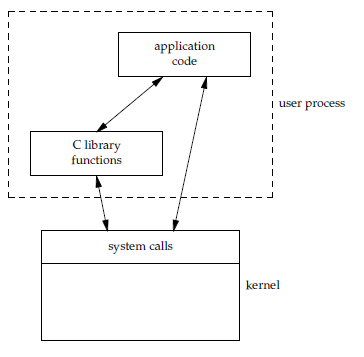
\includegraphics[scale=0.4]{system.png}\\[2pt]
Figure 3: Difference between C library functions and system calls.

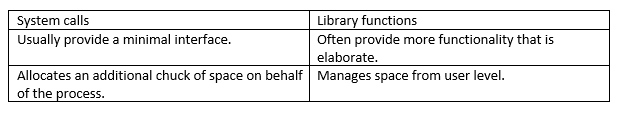
\includegraphics[scale=0.5]{diff.png}\\[2pt]
Figure 4: some of the differences between C library functions and system calls.



\end{frame}

\begin{frame}[t]{SYSTEM CALLS AND LIBRARY FUNCTIONS}
From \textbf{an implementer's point of view,} the distinction between a system call and a library function is fundamental. Unlike \textbf{a user}, for the implementer, both system calls and library functions appear as normal C functions.  As both exist to provide services for application programs. We can replace the library functions whereas the system calls usually cannot be replaced.\\[6pt]
\textbf{Section 8.13 -} show an implementation of the system function that invokes the basic process control system calls with \textbf{an example in Section 10.18} to handle signals correctly.

\end{frame}



\end{document}
